%%%%%%%%%%%%%%%%%%%%%%%%%%%%%%%%%%%%%%%%%
% Short Sectioned Assignment
% LaTeX Template
% Version 1.0 (5/5/12)
%
% This template has been downloaded from: http://www.LaTeXTemplates.com
% Original author: % Frits Wenneker (http://www.howtotex.com)
% License: CC BY-NC-SA 3.0 (http://creativecommons.org/licenses/by-nc-sa/3.0/)
% Modified by Alan G. Labouseur  - alan@labouseur.com, and Ryan Munger - ryan.munger1@marist.edu
%
%%%%%%%%%%%%%%%%%%%%%%%%%%%%%%%%%%%%%%%%%

%----------------------------------------------------------------------------------------
%	PACKAGES AND OTHER DOCUMENT CONFIGURATIONS
%----------------------------------------------------------------------------------------

\documentclass[letterpaper, 10pt]{article} 

\usepackage{tikz}
\usetikzlibrary{automata, positioning}
\usepackage[english]{babel} % English language/hyphenation
\usepackage{graphicx}
\usepackage[lined,linesnumbered,commentsnumbered]{algorithm2e}
\usepackage{listings}
\usepackage{float}
\usepackage{fancyhdr} % Custom headers and footers
\pagestyle{fancyplain} % Makes all pages in the document conform to the custom headers and footers
\usepackage{lastpage}
\usepackage{url}
\usepackage{xcolor}
\usepackage{titlesec}
\usepackage{ulem}

% Stolen from https://www.overleaf.com/learn/latex/Code_listing 
\definecolor{codegreen}{rgb}{0,0.6,0}
\definecolor{codegray}{rgb}{0.5,0.5,0.5}
\definecolor{codepurple}{rgb}{0.58,0,0.82}
\definecolor{backcolour}{rgb}{0.95,0.95,0.92}

\lstdefinestyle{mystyle}{
    backgroundcolor=\color{backcolour},   
    commentstyle=\color{codegreen},
    keywordstyle=\color{magenta},
    numberstyle=\tiny\color{codegray},
    stringstyle=\color{codepurple},
    basicstyle=\ttfamily\footnotesize,
    breakatwhitespace=false,         
    breaklines=true,                 
    captionpos=b,                    
    keepspaces=true,                 
    numbers=left,                    
    numbersep=5pt,                  
    showspaces=false,                
    showstringspaces=false,
    showtabs=false,                  
    tabsize=2
}
\lstset{style=mystyle, language=c++}


\fancyhead{} % No page header - if you want one, create it in the same way as the footers below
\fancyfoot[L]{} % Empty left footer
\fancyfoot[C]{page \thepage\ of \pageref{LastPage}} % Page numbering for center footer
\fancyfoot[R]{}

\renewcommand{\headrulewidth}{0pt} % Remove header underlines
\renewcommand{\footrulewidth}{0pt} % Remove footer underlines
\setlength{\headheight}{13.6pt} % Customize the height of the header

%----------------------------------------------------------------------------------------
%	TITLE SECTION
%----------------------------------------------------------------------------------------

\newcommand{\horrule}[1]{\rule{\linewidth}{#1}} % Create horizontal rule command with 1 argument of height

\title{	
   \normalfont \normalsize 
   \textsc{CMPT 432 - Spring 2025 - Dr. Labouseur} \\[10pt] % Header stuff.
   \horrule{0.5pt} \\[0.25cm] 	% Top horizontal rule
   \huge Lab 3 -- Parsing \\     	    % Assignment title
   \horrule{0.5pt} \\[0.25cm] 	% Bottom horizontal rule
}

\author{Ryan Munger \\ \normalsize Ryan.Munger1@marist.edu}

\date{\normalsize\today} 	% Today's date.

\begin{document}

\maketitle % Print the title

%----------------------------------------------------------------------------------------
%   CONTENT SECTION
%----------------------------------------------------------------------------------------

% - -- -  - -- -  - -- -  -
\section{Crafting a Compiler}
\subsection{4.7 -- Derivations}	
A grammar for infix expressions follows: \\
\begin{figure}[h]
    \centering
    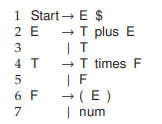
\includegraphics[width=0.35\linewidth]{4-7_grammar.png}
    \caption{Grammar for 4.7}
    \label{fig:enter-label}
\end{figure} \\
(A) Show the leftmost derivation of the following string: [num plus num times num plus num \$]\\
Start \newline
E \$ \newline
T plus E \$\newline
F plus E \$\newline
num plus E \$\newline
num plus T plus E \$\newline
num plus T times F plus E \$\newline
num plus F times F plus E \$\newline
num plus num times F plus E \$\newline
num plus num times num plus E \$\newline
num plus num times num plus T \$\newline
num plus num times num plus F \$\newline
num plus num times num plus num \$\newline

\noindent
(B) Show the rightmost derivation of the following string: [num times num plus num times num \$]\\
Start \newline
E \$\newline
T plus E \$\newline
T plus T \$\newline
T plus T times F \$\newline
T plus T times num \$\newline
T plus F times num \$\newline
T plus num times num \$\newline
T times F plus num times num \$\newline
T times num plus num times num \$\newline
F times num plus num times num \$\newline
num times num plus num times num \$\newline



\subsection{5.2c -- Recursive Descent Parser}
(C) Construct a recursive-descent parser based on the grammar below (psuedo code only) \\
\begin{figure}[h]
    \centering
    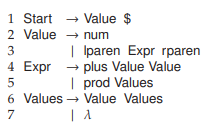
\includegraphics[width=0.5\linewidth]{5-2c_grammar.png}
    \caption{Grammar for 5.2c}
    \label{fig:enter-label}
\end{figure} \\
\newpage
\begin{verbatim}
struct Tree {
    ...
}

func (tree Tree) moveUp() {
    tree.current = tree.current.parent
}

struct Node {
    ... 
}

func match(expected) {
    if currentTok == expected {
        addNode(leaf, x)
    } else {
        err
    }
    currentTokIdx++
    currentTok = tokens[currentTokIdx]
}

var tree Tree = Tree{}
var tokens []Token = []Token{}
var currentTok Token
var currentTokIdx int = 0
currentTok = tokens[currentTokIdx]

func start() {
    parseValue()
    match($)
}

func parseValue() {
    if currentTok == num {
        match(num)
    } else if currentTok == lparen {
        match(lparen)
        parseExpr()
        match(rparen)
    } else {
        err
    }
    tree.moveUp()
}

func parseExpr() {
    if currentTok == plus {
        match(plus)
        parseValue()
        parseValue()
    } else if currentTok == prod {
        match(prod)
        parseValues()
    } else {
        err
    }
    tree.moveUp()
}

func parseValues() {
    if currentTok == num || currentTok == lparen {
        parseValue()
        parseValues()
    } else {
        /* Epsilon */
    }
    tree.moveUp()
}
\end{verbatim}



\section{Dragon Book}
\subsection{4.2.1 A, B, C -- Derivations and Parse Trees}
Consider the grammar $S \to S S + | S S * | a$ and the string aa+a*. \\
(A) Give a leftmost derivation for the string. \\
S \newline
SS* \newline
SS+S* \newline
aS+S* \newline
aa+S* \newline
aa+a* \newline
\\
(B) Give a rightmost derivation for the string. \\
S \newline
SS* \newline
SS+S* \newline
SS+a* \newline
Sa+a* \newline
aa+a* \newline
\newpage
\noindent
(C) Give a parse tree for the string. \\
\begin{verbatim}
S
-S
--S
---a
--S
---a
--+
-S
--a
-*
\end{verbatim}

\end{document}